
%!TeX spellcheck = en-US
%\chapter{Word Embedding and Distributional Features of the web-pages and texts}
\chapter{The Usefulness of Distributed Representation in WGI}

\label{chap:word_embeddings}


%----------------------------------------------------------------------------------------

% Define some commands to keep the formatting separated from the content
\newcommand{\keyword}[1]{\textbf{#1}}
\newcommand{\tabhead}[1]{\textbf{#1}}
\newcommand{\code}[1]{\texttt{#1}}
\newcommand{\file}[1]{\texttt{\bfseries#1}}
\newcommand{\option}[1]{\texttt{\itshape#1}}

%----------------------------------------------------------------------------------------

\section{Introduction}\label{chap:word_embeddings:sec:intro}
 
The most traditional text representation scheme in text mining tasks is the Bag of Words (BOW) model which is based on individual tokens as features. It is a simplistic approach to quantify information documents assuming independence of the occurrence of individual tokens in documents. The result is a document vector of high dimensionality (i.e., in the order of thousands of features) and sparseness (i.e., only a few non-zero values per document). The BOW model is not able to capture information about the grammar of documents and completely ignores word order. In addition, it is confused by synonym terms since it assumes they are independent. Nevertheless, it provides an easy and quite competitive approach to represent documents (the W1G scheme used in Chapter \ref{chap:noise} is actually based on BOW).

A more elaborate text representation scheme is to consider n-gram of words. This would capture information about word sequences, like phrases. This can improve the ablity of the model to represent syntactic information since the context of words is partially taken into account (e.g., the W3G model used in Chapter \ref{chap:noise}). Nevertheless, the dimensionality of representation is considerably increased when the order of the model ($n$) is high. In addition, the sparseness of the vectors is increased. It is also possible to apply the n-gram approach on the character level or on POS-tag level, as shown in the experiments of Chapter \ref{chap:noise} (i.e., C4G, POS3G). The main assumption that each feature (n-gram) is independent of the other features is still valid in such models.

An alternative approach is to use \textit{distributed representations} that attempt to introduce some kind of dependence of each word (or n-gram) on the other words (or n-grams). For example, the words usually encountered in the context of a specific word are more dependent on that word. In addition, different words found in similar context get a higher share of dependence. Distributed representations can be obtained by applying language modeling methods. Especially, the use of neural network language models and the popular word and document \textit{embeddings} introduced in \parentcite{mikolov2013distributed}. 

One main advantage of distributed representations is that they provide compact (i.e., low-dimensional) and dense vectors to quantify syntactic and semantic information in documents. In comparison to regular BOW or n-gram models, distributed features are much less redundant and irrelevant since each such feature captures a combination of information that cannot be specifically determined. Therefore, it seems that open-set WGI methods that are not able to easily handle high-dimensional, sparse vectors with many irrelevant and redundant features would be highly improved by using distributed representations. As already explained in Chapter \ref{chap:openset}, NNDR is an algorithm that, in theory, is vulnerable when it is not combined with appropriate feature sets. The main goal of this Chapter is to examine how the performance of NNDR in WGI tasks can be improved when distributed features are used. 

The rest of this chapter is organized as follows. First, the main ideas of distributed representation are presented. Then, the specific distributed features used in this thesis are described. Next, we compare the performance of NNDR using traditional sparse representation schemes with the case dense vectors are used. We also compare these versions of NNDR with OCSVM and RFSE methods and discuss the main conclusions of this study.

\section{Obtaining Distributed Representations}

%The SLM model is defined as the \textit{joint conditional probability distribution} of the next word given the probabilities of previous ones as shown in equation \ref{chap:word_embeddings:eq:slm}

%\begin{equation} \label{chap:word_embeddings:eq:slm}
%	P(w = i) = \prod_{i=1}^{|V|} P(w_{i}|w_{i-k}, ... , w_{i+k})
%\end{equation}
%\noindent
%where $w_{i}$ is the i-th word, and $k$ is for the number of words before or/and and after, writing sub-sequence $w_{i} = (w_{i-k}, w_{i-1}, ... ,w_{i+1}, w_{i+k})$. Note that this model returns a singleton value for a word on the condition of previews or/and next word. This model also can be expanded to have few more words in the conditional probability, usually from 2 up to 4. 

%With this model it can be captured the semantic proximity but it will return zero in the case a sequence have never been met before in the samples. A solution to this problem is the interpolation or smoothness factor that can be applied such as in the \textit{back-off}  model (Katz, 1980 see in bengio2003neural). 

%The model of equation \ref{chap:word_embeddings:eq:slm} can capture the joint probability of word-sequences in terms of feature vectors, however, it cannot capture the correlation of the words in terms of semantics. Models like LSI or LDA are methodologies also been tested in IR and NLP for capturing the semantics in the context of the n-gram based SLM. 

One way to obtain a low-dimensional and dense representation of documents is the use of topic modeling. Topic modeling methods attempt to group terms according to their co-occurrence in documents. They provide a new feature space (composed by latent topics) of pre-defined dimensionality. One popular topic modeling approach is \textit{Latent Semantic Analysis}, a linear algebraic method that transforms a high-dimensional and sparse representation to a low-dimensional and dense one applying \textit{singular value decomposition} \parentcite{Kontostathis:2006}. Another popular approach is \textit{Latent Dirichlet Allocation}, a generative probabilistic where each documents is represented as a mixture over a set of latent topics. Each topic is in turn defined as a distribution over words \parentcite{Blei:2003}.

Another main direction that gained huge popularity during the last years is the use of neural probabilistic language models \parencite{bengio2003neural}. We first describe how words can be represented in a coninuous space and then we focus on documents.

\subsection{Word Embeddings}

The main idea is that words can be represented by real vectors (word embeddings) that are learned by a neural network \parentcite{mikolov2013efficient}. This is unsupervised learning since documents need not be labeled. The neural network is trained to recognize words that occur in similar context. Then, each word is represented in continuous vector space and similar words tend to cluster in the same area. In addition, the distance between related words is affected by semantic similarity (e.g., the difference between terms "king" and "man" is close to the difference between "queen" and "woman") \parentcite{mikolov2013efficient}. 

In practice the distributed features is the mapping of the vocabulary words $V = \{w_{i}, i \in [1, |V|] \}$ to a real vector $\vec{t}_i \in \mathbb{R}^{m}$.

%Then the semantic distance can be approximated by a NNet algorithm given the distribution of the words. The words are initially are having a vector 1-of-V representation, a.k.a. \textit{One-hot representation}. Then the probability of the a word $w_{i}$ in equation \ref{chap:word_embeddings:eq:slm} can be replaced by the real continues vector $t{i}$ and the conditional probability $P(.|.)$ to be approximated my a NNet function $\hat{p}(.)$. The $\hat{}$ (hat) is for symbolizing a special condition where the probability is approximated given a sequence with a specific order, say preceding words or succeeding words or both. 

%Now the DF neural model can be calculated with several architectures where the $\vec{t}$ and the $\hat{p}$ continues distribution can feed separate layers of joint layers, and also the learning strategy can have variant implementations such as Continues Bag-of-Words, Skip-grams etc. The strategy of learning and the NNet architecture are very close related and the results are \textit{continues probability functions with substantially different meaning}, where they can either encode word similarities, word semantics or even paragraph and documents encoding and similarities. 

One basic architecture is the Continuous Bag-of-Words (CBOW) model which attempts to predict a word given its context. This is a \textit{Feedforward Neural Network} with an input layer, a projection layer, and an output layer as shown in figure \ref{chap:word_embeddingss:fig:CBOW_diagram}. The input layer is composed by the context of a word (i.e., the few words immediately to its right and left). Every word in the vocabulary is assigned to a \textit{one-hot} vector $\hat{t}_{i}$ (i.e., a vector of size $|V|$ with all but one values equal to zero). The sequence of context word vectors are added and form the input vector $\hat{t}_{i*}$. Since the order of words is not important in this setting, the model bears similarities to Bag-of-Words \parencite{mitra2018introduction}.

%W_{in}$ is the weight matrix of the projection layer with regularization parameters $\theta$. Now the $\vec{t}$ is the input to a hidden layer $\vec{h}=\vec{t}H$, which is usually the \textit{hyperbolic tangent hidden layer}, where $H$ is the weights of the hidden layer. Then, the output $\hat{p}=\vec{h}W_{out}$ is the last layer of the NNet.

\begin{figure}[t]
	\begin{center}
    	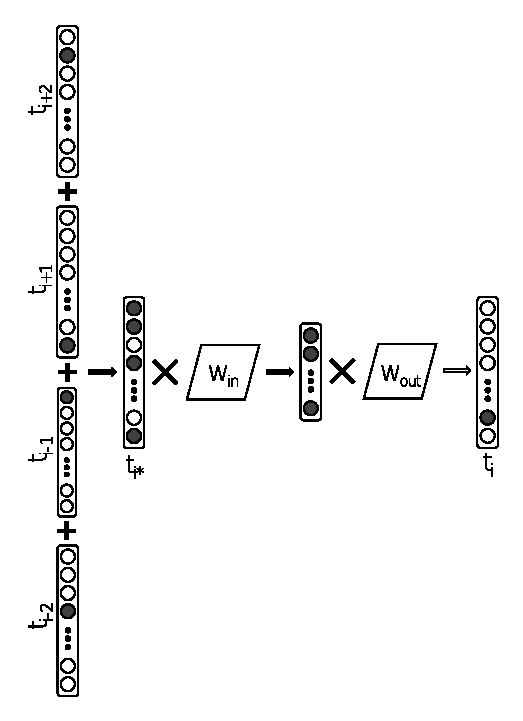
\includegraphics[scale=0.99]{Figures/CBOW_diagram.eps}
		\caption{Diagram for C-BOW and General NLM architecture. Depending whether the $t_{i*}$ is part of the projection and the hidden layer or the layers are different. In practice the weighting matrices are either shared or diff rent between the word projection and the hidden layer or it is the same matrix, which is equivalent to the words been projected to the same position as their vectors are averaged and not concatenated.}
		\label{chap:word_embeddingss:fig:CBOW_diagram}
	\end{center}
\end{figure}

%The generic architecture of the final output of the NLM described above is the equation \ref{chap:word_embeddingss:nlm_generic}. Note that the output vector $\vec{y}$ has size $|V|$ due to the input $\hat{w}$ and is the inference model of a \textit{continues distribution} of both the proximity of the words in the sentences (captured by the hidden layer) and the distribution over the vocabulary, which is the continues similarity of the words in this vocabulary. The output layer then is as described in equation \ref{chap:word_embeddings:eq:NLM}

%\begin{equation} \label{chap:word_embeddings:eq:NLM}
%	\vec{y} = \vec{t} + W_{out}(\vec{t}H + b_{h}) + b_{o}
%\end{equation}

%\noindent
%where $b_{o}$ and $b_{h}$ are the output and hidden layers biases. Usually the Hidden layer typically has a size of 500 to 1000 neurons while the projection layer might be 500 to 2000. Due to the multiple layers and the feeding of both the projection and the hidden to the output layer there is great complexity and the process is very computationally demanding. 

%A more efficient method is suggested in \parencite{mikolov2013efficient} where the non-linear hidden layer is removed and the projection layer is shared to all words, geometrically this is equivalent to the projection of the words to the same position. Then the algorithm is reformed and the $\hat{w}$ vectors are replaced by the $t^{*}$ which is the sum of the \textit{one-hot word vectors} \parencite{mitra2018introduction}. 

%Now the equation \ref{chap:word_embeddings:eq:NLM} is becoming \ref{chap:word_embeddings:eq:CBOW}. Due to the new form of the NNet where the tangent hidden layer is absent, there is no constraint in the presenting sequence of the words order. Moreover, the succeeding words also can also be taken in to account in a given \textit{window} say for $k_{w}$ number of words around the specific one. 

The weight matrix $W_{in}$ is of size $|V| \times m$ while $W_{out}$ is of size $m \times |V|$, where $m$ is the size of the hidden layer ($m << |V|$) and it also corresponds to the dimensionality of the extracted distributed representation. The size of the output vector is equal to the vocabulary size. 
%
%\begin{equation} \label{chap:word_embeddings:eq:CBOW}
%	\vec{y} = \hat{t}_{i*} \times W_{out} + b_{o}
%\end{equation}

During training, CBOW attempts to learn weight matrices $W_{in}$ and $W_{out}$. The loss function of CBOW is the following conditional log probability: 

\begin{equation} \label{chap:word_embeddings:eq:CBOW_log_likelihood}
	 \mathcal{L}_{CBOW} = -\frac{1}{|S|} \sum_{i=1}^{|S|}{\log{p(t_{i}|t_{i-k}, ... ,t_{i+k})}}
\end{equation}

\noindent
where $k$ is the size of context words, $S$ is the amount of possible context windows. \textit{Stochastic Gradient Decent} and \textit{Backpropagation} are used to train that network. CBOW is actually a encoder-decoder model and applies a \textit{SoftMax} function in its output: 

\begin{equation} \label{chap:word_embeddings:eq:CBOW_softmax}
	p(t_{i}|t_{i-k},...,t_{i+k}) = \frac{e^{y_{t_{i}}}}{\sum^{|V|}_{i}{e^{y_{t_i}}}}
\end{equation}

\nointdent where $y_{t_i}$ is the output vector for term $t_i$.

Another architecture is the \textit{skip-gram} model, that attempts to predict the context of a word. This is depicted in figure \ref{chap:word_embeddingss:fig:skipgram_diagram}. Again, input and output are one-hot vectors while the hidden layer is of dimensionality $m$ ($<<|V|$). The objective is to learn weight matrices $W_{in}$ and $W_{out}$ and the loss function is as follows:

\begin{equation} \label{chap:word_embeddings:eq:skipgram_log_likelihood}
	 \mathcal{L}_{SkipGram} = -\frac{1}{|S|} \sum_{i=1}^{|S|}{ \sum_{-k \leq j \leq +k}{ \log {p(t_{i+j}|t_{i})}  } }
\end{equation}

\nointend where $k$ is the number of context words to be predicted, $S$ the number of all windows in training set, and $p(t_{i+j}|t_{i})$ is obtained as follows:

\begin{equation} \label{chap:word_embeddings:eq:skipgram_softmax}
	p(t_{i+j}|t_{i}) = \frac{ e^{(W_{out}  \times  t_{i+j})^{T} (W_{in} \times  t_{i})}}{\sum^{|V|}_{k=1}{ e^{(W_{out}  \times  t_{k})^{T} (W_{in} \times  t_{i})}}} 
\end{equation}

\begin{figure}[t]
	\begin{center} 
    	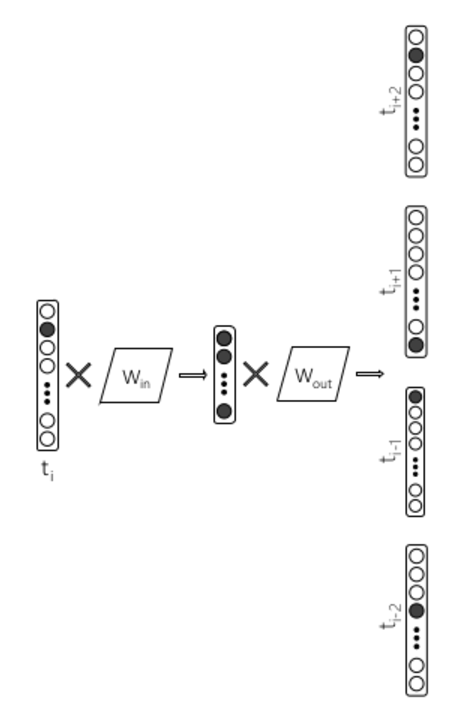
\includegraphics[scale=0.99]{Figures/skip_gram.eps}
		\caption{Diagram for Skip-Gram.}
		\label{chap:word_embeddingss:fig:skipgram_diagram}
	\end{center}
\end{figure}

Finally, the above neural models, either CBOW or skip-grams, since they are approximating the continuous distribution probability function of words over the the Vocabulary $V$ they also satify the following constraint:

\begin{equation} \label{chap:word_embeddings:eq:nnet_condtraint}
	\sum_{i=1}^{|V|}{p(t_{i}|t_{i-k}, ... ,t_{i+k})} = 1
\end{equation}

Note that in both CBOW and skip-gram models the two weight matrices $W_{in}$ and $W_{out}$ can be used to provide the word embeddings\footnote{An implementation of these methods is provided in https://github.com/tmikolov/word2vec}. Usually $W_{in}$ plays this role and $W_{out}$ is discarded.

\textcolor{red}{THIS IS NOT CLEAR: A very important difference between the CBOW and skip-grams is the NNet architecture usually their implementation is based. Particularly, there are some internal detail occurring because of the objective of the task. \parencite{boden2002guide}}

To summarize, the above models are very effective \textit{Language Modeling} approaches having the ability to quantify simultaneously syntanctic and semantic information of words. They provide a \textit{distributed representation} for words (i.e., each word is represented with a dense vector which is a point in a space of relatively low dimensionality). The sequence of words in texts is now considered and can also be applied in cases input texts are composed of seguences of characters or POS tags.

Finally, the training of the CBOW and the skip-gram models can be expensive despite the fact of limiting the number of hidden layers. However, there are several engineering solution that are accelerating the training time, such as \textit{Huffman binary Tree encoding} of words and \textit{hierarchical soft-max}. The latter is a solution that enables us to use multi-processing power and update the weight parameters concurrently. The parallel asynchronous updating of the parameter matrices is not conforming to the mathematical constraints however in practice the negative effect is minor. Huffman binary tree is a method for compressing the encoding of terms where the ones with the higher frequency are accessed faster. In addition to this, \textit{negative sampling}, \textit{sub-sampling}, or \textit{ramdom sampling} are also used where in the range of $k$ window for surrounding words only a few are selected during training with minor effect in  performance and significant acceleration in training \parentcite{mikolov2013efficient,mitra2018introduction}. 

\subsection{Document Embeddings} \label{chap:word_embeddings:sec:PVBOW} 
 
There are several approaches to tranform word embeddings to document embeddings \parencite{mitra2018introduction,mikolov2013distributed}. The most simple method produces a vector for a given document by averaging the word embeddings of the words in a document. It is also possible is to modify the network architecture and work on the sentence level. For example, word embeddings per sentence are averaged and the goal is to predict a sentence given its context sentences \parentcite{Kenter:2016}. Another idea, the \textit{Sent2Vec} method, is to compose sentence embeddingsby extending CBOW to include word vectors and word n-gram embeddings \footnote{An implementation of this method can be found in https://github.com/epfml/sent2vec}.

In this thesis, we use the \textit{Doc2Vec} approach introduced in \parentcite{le2014distributed}. that attempts to generalize the word embeddings methods to work with sequences of words. 


In this study, the Paragraph Vector Bag-of-Words (PV-BOW) model is used for the WGI task in the open-set framework evaluation. The PV-BOW is a DF modeling of the documents as an extension of the Skip-Grams modeling. The PV-BOW extends the idea of the \textit{Continues Distribution of the Words} over the Vocabulary and the Context defined by a Corpus of documents. A \textit{Continues Distribution of the Paragraphs (CDP} is defined where this method considers the concatenation of the paragraph vector with the word vectors to predict the next word in a text window. 
 
The CDP can be derived with two methods, one is based on CBOW and the other on Skip-Grams, which is used in this study. The CBOW extension is called Distributed Memory Paragraph Vector (PV-DM) because the Paragraph Vector is given as an input together with the word vectors, and it is considered as memory of the words distribution.
 
Another way is to ignore the context words in the input, and make a model for predicting words randomly sampled from the paragraph in the output. That is the Skip-gram model but instead of a words the whole paragraph vector is given as an input as shown in figure \ref{chap:word_embeddingss:fig:PVBOW_diagram}. In practice, at each iteration of stochastic gradient descent, text window of $k$ size is sampled. Then a random word sampled from the text window and form a classification task given the Paragraph Vector and  this is the PV-DBOW. This model requires to store less data, because only the softmax weights are stored as opposed to both softmax weights and word vectors in the PV-DM. 

\begin{figure}[t]
	\begin{center} 
      	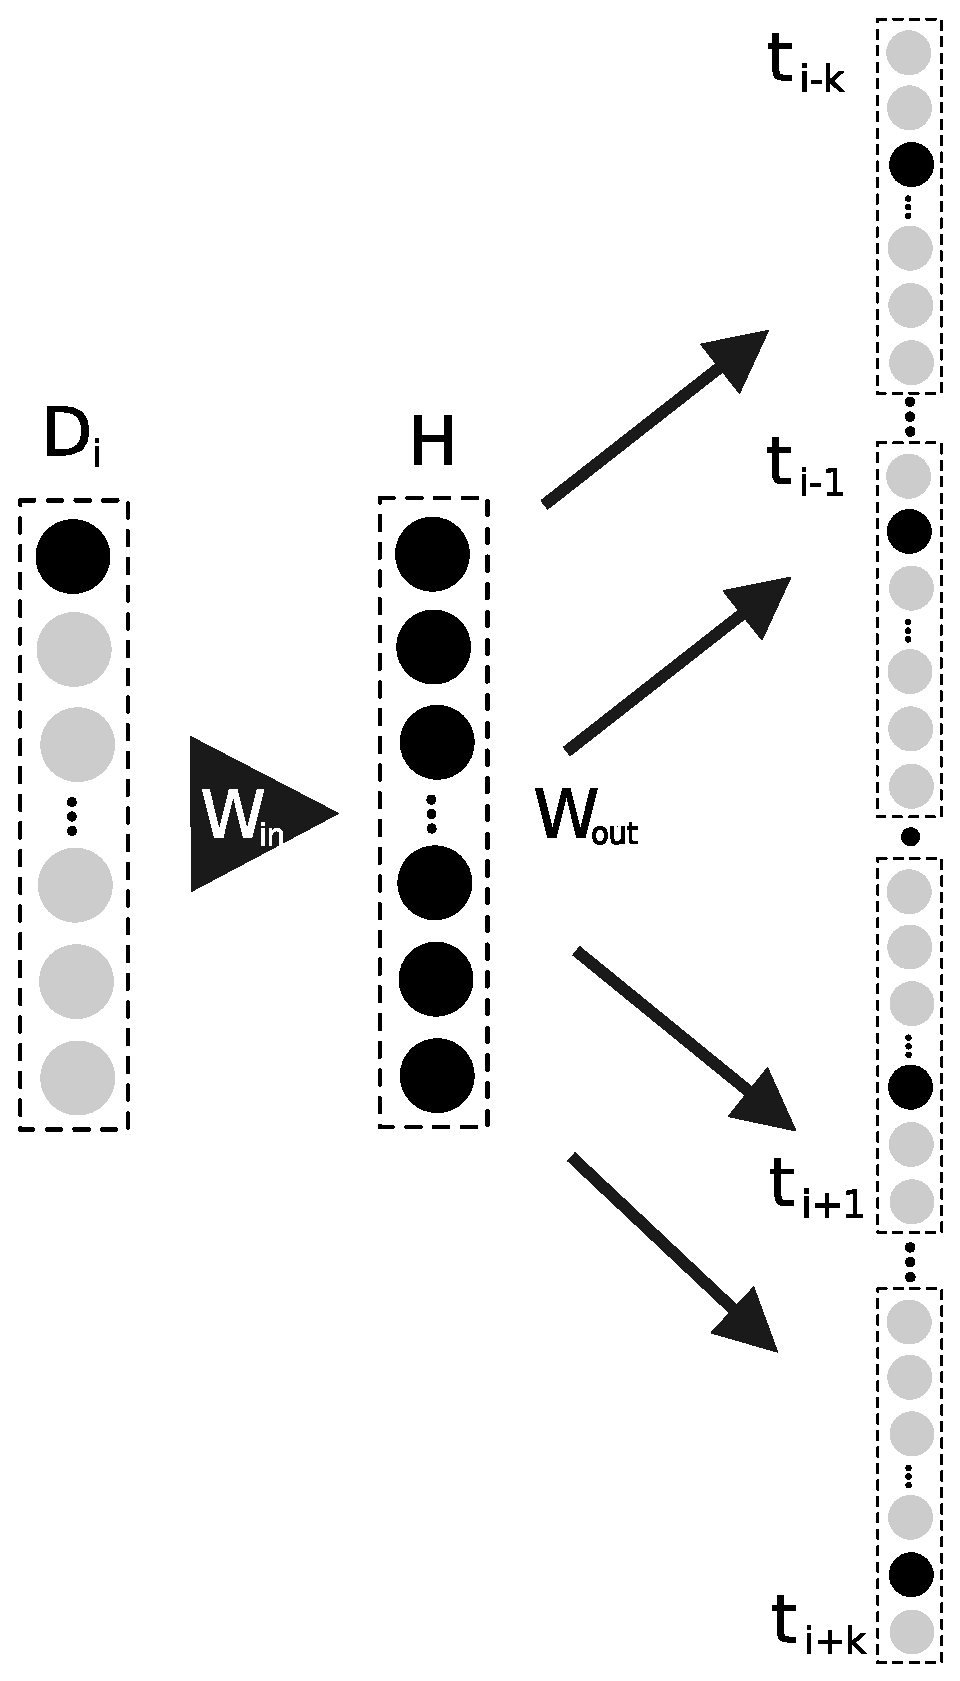
\includegraphics[scale=0.50]{Figures/pvbow.eps}
    		\caption{Diagram for PV-BOW}
		\label{chap:word_embeddingss:fig:PVBOW_diagram}
	\end{center}
\end{figure}


It should be noted that the Paragraph Vectors can be a text paragraph, a sentence, or the whole document. In this study, the whole web-pages is considered as shown in the first vector at the left in figure \ref{chap:word_embeddingss:fig:PVBOW_diagram}. There are several implementation for the PV-BOW modeling and a late evolution proposal for making the model more appreciate for IR problems. Including, \textit{Document frequency based Negative Sampling} and \textit{Document Length Regularization} \parencite{le2014distributed,posadas2017application}.

The PV-BOW objective log likelihood of Skip-gram models described in equation \ref{chap:word_embeddings:eq:skipgram_log_likelihood} is changing to the equation \ref{chap:word_embeddings:eq:pvbow_log_likelihood}  

\begin{equation} \label{chap:word_embeddings:eq:pvbow_log_likelihood}
	 \mathcal{L}_{SkipGram} = \frac{1}{|S|} \sum_{i=1}^{|S|}{ \sum_{-k \leq j \leq +k}{ \log {p(t_{i+j}|D_{i};\theta)}  } }
\end{equation}
\noindent
where $D_{i}$ is the Document Vector or Document ID, $S$ is the prediction windows over the training text and $k$ is the number of the words to be predicted surrounding the input word $\theta$ set of parameters to be optimized. Consequently,  the Softmax function is becoming as shown in equation \ref{chap:word_embeddings:eq:pvbow_softmax}.

\begin{equation} \label{chap:word_embeddings:eq:pvbow_softmax}
	p(t_{i+k}|t_{i}) = \frac{ e^{(W_{out}  \times  t_{i+j})^{T} (W_{in} \times  D_{i})}}{\sum^{|V|}_{i}{ e^{(W_{out}  \times  t_{k})^{T} (W_{in} \times  D_{i})}}} 
\end{equation}
Paragraph Vectors address some of the key weaknesses of bag-of-words (remember words can be any terms characters, words or POS) models. First, they capture the semantics of the terms. Therefore, words like “strong”  and "powerful" are closer together both and far from "Athens". Secondly, paragraph vectors take into consideration the word order, at least in sentence or paragraph level, in the same way that an Word n-Gram model would do in the size of n-Terms. As we will see experimentally the n-gram model also preserves a lot of information of the paragraph such as the word order. However, even if in some cases like in the experiments below, the n-grams perform equally to the PV-BOW DF models, the DF models can generalize better. They encoding more information with much denser and continuous dimemnsionality or at least the information they capture is not sparse and maybe "broken" in the small ranges of n-terms.

In practice a library for HTML reprocessing and and Vector Representation of the web-pages has been created for this work, named  \textit{Html2Vec}\footnote{\url{https://github.com/dpritsos/html2vec}}. There as special module for PV-BOW modeling has been build, where it is based on the the algorithm can be found at \textit{Gensim package} \footnote{\url{https://github.com/RaRe-Technologies/gensim}}. 


In this study a PVBOW Distributional Feature model for the whole corpus is trained. The corpus initially is split to a set of paragraphs, as required from PVBOW. To be more specific the paragraphs are sentences split from all the document of the whole corpus. Then several models PVBOW feature models are trained for a variety of parameters and vector dimensions, explained in the experiments section below. After the model has been fitted then one vector for each web-document was inferred from the PVBOW. The final document vectors derived from \tetxit{Distributional Feature Model} are given to the open-set learning model explained below. 


\section{Experimental Setup}\label{chap:word_embeddings:sec:experiments_setup}

%\subsection{Corpus}\label{chap:word_embeddings:sec:experiments_corpora}

The experiments of this chapter, are based on \textit{SANTINIS}, a benchmark corpus already used in previous work in WGI \parencite{mehler2010genres_on_web,pritsos2018open,santini2007automatic}. Briefly, this dataset comprises 1,400 English web-pages evenly distributed into seven genres (blog, eshop, FAQ, frontpage, listing, personal home page, search page) as well as 80 BBC web-pages evenly categorized into four additional genres (DIY mini-guide, editorial, features, short-bio). In addition, the dataset comprises a random selection of 1,000 English web-pages taken from the SPIRIT corpus \parencite{joho2004spirit}. The latter can be viewed as \textit{unstructured noise} since genre labels are missing. More details for SATNINIS corpus are discussed in section \ref{}. 


%\subsection{Open-set Models Parameters Setup}\label{chap:word_embeddings:sec:experiments_params}

To represent web-pages again the features are exclusively related to textual information, excluding any structural information, URLs, etc. The following representation schemes are examined: Character 4-grams (C4G), Word unigrams (W1G), and Word 3-grams (W3G). For each of these schemes, we use either Term-Frequency (TF) weights or DF features. The feature space for TF is defined by a vocabulary $V_{TF}$, which is extracted based on the most frequent terms of the training set --- we consider $V_{TF}=\{5k,10k,50k,100k\}$. The DF space is pre-defined in the PV-BOW model --- we consider $DF_{dim}=\{50,100,250,500,1000\}$.

In PV-BOW, the terms with very low-frequency in the training set are discarded. In this study, we examine $TF_{min}=\{3,10\}$ as cutoff frequency threshold. The text window size is selected from $W_{size}=\{3,8,20\}$. The remaining parameters of PV-BOW are set as follows: $\alpha=0.025$, $epochs=\{1, 3, 10\}$ and $decay=\{0.002, 0.02\}$. The PV-BOW creation process is also driven by an internal terms \textit{vocabulary} which is used for eliminating the terms with lower than a preferred frequency and then discards the terms from the text window for the PV-BOW (see section \ref{}).


Regarding the NNRD open-set classifier, there are two parameters, $lambda$ and DRT, and their considered values are: $\lambda =\{0.2, 0.5, 0.7\}$, $DRT\textit{=\{0.4, 0.6, 0.8, 0.9\}}$. All aforementioned parameters are adjusted based on grid-search using only the training part of the corpus.

For a proper comparison with prior art, the Random Feature Subset Ensemble (RFSE) and one-class SVM (OCSVM) \parencite{pritsos2013open,pritsos2018open} are used as baseline, the two open-set WGI approaches with good results presented in chapter \ref{chap:noise}. All parameters of these methods have been been adjusted as suggested in this section (for the same corpus).

The open-set evaluation framework is followed with \tetxit{unstructured noise} introduced in the preview section \ref{}. In particular, the open-set F1 score \parencite{mendesjunior2016} is calculated over the known classes (the noisy class is excluded). The reported evaluation results are obtained by performing 10-fold cross-validation and, in each fold, the full set of 1,000 \tetxit{noise pages} was included. 

This evaluation strategy is giving a more realistic evaluation. Since the noise size is greater than the size of any genre included in the given genres collection.

To compensate the unbalanced distribution of web pages over the genres because of the noise part, the macro-averaged precision and recall measures is used as explained in section \ref{} and also used in \parencite{mendesjunior2016}. Note again than this special modified method calculates precision and recall only for the known classes (available in the training phase) while the unknown samples (belonging to classes not available during training) affect false positives and false negatives. 

Finally, for selection parameter settings that obtain optimal evaluation performances the two scalar measures are used where their usage is reasoned in section \ref{}. Firstly, the \textit{Area Under the Precision-Recall Curve} (AUC) to the  standard \textit{11 Recall Levels} and particularly the Macro-AUC (MAUC). Secondly, the $F_{1}$ and specifically the Macro-F1 (MF1) score.


\section{Experimental Results}\label{chap:word_embeddings:sec:results}

\subsection{NNDR with DF or TF Features}\label{chap:word_embeddings:sec:NNDR_PVBOW_vs_BOW}

NNDR, analytically described in \ref{}, is an open-set formation of the NN algorithm. On the contrary to the previously discussed open-set algorithms such as the RFSE, it has the ability to explicitly parameterized for regulating the \textit{open space risk}. In this paragraph the NNRD performance is evaluated in the open-set with \textit{unstructured noise} conditions, using the SANTINIS corpus.

Additionally, since the noise-class is marked the algorithm is evaluated in both false-positive and the false-negative classifications of the marked-unknown-classes. The Macro-F1 and Macro-PRC are capturing the this error an penalizing the performance of the algorithm when this happens, as also explained in section\ref{} chapter 4.

Initially NNDR is evaluated in the BOW features with TF weighting schema vocabulary as shown in table \ref{chap:word_embeddings:tbl:NNDR_TF}. The overall performance is poor, however, better to the OCSVM's performance in table \ref{}, of section \ref{}. Constantly, to the experiments of chapter \ref{} the W3G is the \textit{terms type} where NNDR can have MAUC and MF1 over $0.66$. The algorithms parameters are also slightly affected for STP and SUP, while DRT in all cases is $0.8$. The $\lambda$ parameter has no effect, i.e. can be any value of the available set of these experiments. In should also be noted that the MF1 and the MAUC are both maximized for the same document representation, i.e. W3, the same vocabulary size, i.e. 10000, and the same algorithm parameters.

\begin{table}
\center
\begin{tabular}{cccclrrrrr}
\hline
STP & SUP & DRT & $\lambda$ & T.TYPE & DIMs & M\emph{P} & M\emph{R} & M\emph{AUC} & M\emph{F1} \\
\hline
0.7 & 0.3 & 0.8 & any & C4G & 5000 & 0.664 & 0.403 & 0.291 & 0.502 \\
0.7 & 0.5 & 0.8 & any & W1G & 5000 & 0.691 & 0.439 & 0.348 & 0.537 \\
0.5 & 0.5 & 0.8 & any & W3G & 10000 & 0.720 & 0.664 & 0.486 & 0.691 \\
\hline
\end{tabular}
\caption {Maximum performance of NNDR on TF Features of SANTINIS coprus. STP is the Spliting Training Percentage. SUP is the Splitting Unknown Percentage. DRT is the Distance Ration Threshold. $\lambda$ is the weigthing balance regulation parameters for the Normalized Accuracy. T.TYPE is the Terms Type. DIMs is the features model's dimensions. MP is the Macro Precision. MR is the Macro Recall. MAUC is the Area Under the Macro PR Curve. MF1 is the F1 score of the Macro Precision and Macro Recall.}
\label{chap:word_embeddings:tbl:NNDR_TF}
\end{table}



\begin{table}
\center
\begin{tabular}{cccclrrrrr}
\hline
STP & SUP & DRT & $\lambda$ & T.TYPE & DIMs & M\emph{P} & M\emph{R} & M\emph{AUC} & M\emph{F1} \\
\hline
any & any & 0.8 & any & C4G & 50 & \textbf{0.829} & 0.600 & 0.455 & 0.696 \\
any & any & 0.8 & any & W1G & 50 & 0.733 & 0.670 & 0.541 & 0.700 \\
any & any & 0.8 & any & W3G & 100 & 0.827 & 0.615 & 0.564 & \textbf{0.706} \\
\hline
\end{tabular}
\caption {Maximum performance of NNDR on Distributional Features of SANTINIS corpus. STP, SUP, DRT, $\lambda$, T.TYPE, DIMs are the same as in table \ref{tbl:NNDR_TF}. MTF is the Minimum Threshold Fequency of the Distributional models Vocabulary. WS is the Windows Size of the text sentence. $\alpha$ is the NNet parameter. EP is the epochs number of the NNet model. DEC is the decay parameter of the NNet model. MP is the Macro Precision. MR is the Macro Recall. MAUC is the Area Under the Macro PR Curve. MF1 is the F1 score of the Macro Precision and Macro Recall.}
\label{chap:word_embeddings:tbl:NNDR_PVBOW}
\end{table}

In the next evaluation step the NNDR has been tested using the PVBOW \textit{distributional features neural model }as described in section \ref{chap:word_embeddings:sec:PVBOW}. As shown in table \ref{chap:word_embeddings:tbl:NNDR_PVBOW} the performance of the algorithm has a significant improvement since the  MF1 from $0.691$ climbs to $0.706$ with the lowest performance at $0.696$ for C4G. It also should be noted that the is also maximized for the same parameters. 

The NNRD consistently returns is highest performance with the W3G for PVBOW model and for BOW TF vectors. The PVBOW seems to improve the $MP$ significantly by reaching the score of $0.829$ comparing to the initial maximum of $0.720$, with BOW. On the contrary to the BOW the maximum precision is returned with C4G while the maximum MF1 is returned for W3G. However, the precision score returned for W3G is very close to the one of C4G.

The PRC diagram is shown in figure  \ref{chap:word_embeddings:fig:NNDR_W3G} for having a better insight of the NNDR algorithm's improvement with the PVBOW neural language model compare to the BOW with TF weighting scheme. In particular, the W3G document representation is used for both diagrams of the NNDR because in both cases the $MACU$ and the MF1 are both maximized for either BOW or PVBOW.

\begin{figure}[H]

\begin{center}
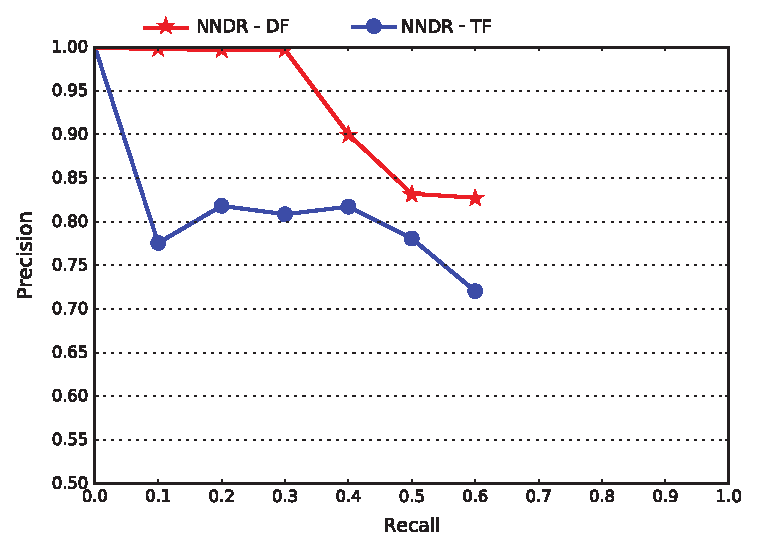
\includegraphics[scale=0.99]{Figures/NNDR_W3G.eps}
\caption{Precision-Recall Curves of NNDR on SANTINIS corpus. The curves are for W3G terms-type and for AUC optimization criterion. The 11-recall-levels are shown for each evaluation experiment. The lines are stopping before the 11th recall level due to the open-set framework, i.e. the remaining part after the last mark of each curve it the percentage of the corpus tha has been classified as Unknown from the algorithms.}
\label{chap:word_embeddings:fig:NNDR_W3G}
\end{center}

\end{figure}

The NNDR-DF is starting higher than NNDR-TF and it remains to $0.99$ precision for the $30\%$ of the corpus. Then it drops rgradualy and remains over $0.80$ up to $60\%$ of the corpus. The the rest of the corpus is classified as unknown. RFSE manages to recognize correctly part of the corpus up to $80\%$ with the precision to drop to $0.70$ and then to $0.65$. 

Considering the NNDR-TF is significantly lower in performance and for the first $10\%$ of the corpus is just above $0.75$. Given that the curves are calculated based on the ranked scores from the best performance to the lowest performance it seems that the algorithm significantly affected by the \textit{unstructured noise}. That is, the algorithm makes very confident decision for some part of the corpus confusing them with other classes. Its overall performance is over $0.7$ precision and also recognize the $60\%$ of the corpus, just like with the DF.

To conclude it seems that NNDR with distributional features is returning a significantly better performance than the BOW with TF weighting scheme. Although the $ΜR$ for PVBOW is slightly lower comparing the last row of both tables \ref{chap:word_embeddings:tbl:NNDR_TF} and \ref{chap:word_embeddings:tbl:NNDR_PVBOW}, the $MP$ is significantly higher. This is more important especially for the task o WGI in an open-set framework with noise, as explained in detail previously (see section \ref{}) in this thesis. 

In the next section the NNDR is compared to the RFSE and OCSVME open-set algorithms both described in \textit{chapter \ref{chap:openset}} and their evaluation experiments presented in \textit{chapter \ref{chap:noise}}.


\subsection{Comparison of Open-set WGI Methods}\label{chap:word_embeddings:sec:experiments_setup}

In this section the objective is to find out  how far the improvement of an open-set algorithm can go with the PVBOW neural language model compare to the RFSE and OCSVME as baselines. The baselines and NNDR are applied in the SANTINIS corpus. 

In the training phase, only the 11 known genre classes are use, while in test phase an additional class of the \textit{unstructured noise} is considered. Table\ref{chap:word_embeddings:tbl:NNDR_RFSE_OCSVME_final} shows the performance of tested methods when either TF or DF representation schemes, based on C4G, W1G, or W4G features, are used. 

\begin{table}[t]
\center
\caption {Performance of baselines and NNDR on the SANTINIS coprus. All evaluation scores are macro-averaged.}
\label{chap:word_embeddings:tbl:NNDR_RFSE_OCSVME_final}
\begin{tabular}{ccccccc}
\hline
Model & Features & Dim. & Precision & Recall & AUC & F1 \\
\hline
RFSE & TF-C4G & 50k & 0.739 & \textbf{0.780} & 0.652 & 0.759 \\
RFSE & TF-W1G & 50k & 0.776 & 0.758 & \textbf{0.657} & \textbf{0.767} \\
RFSE & TF-W3G & 50k & 0.797 & 0.722 & 0.615 & 0.758 \\
OCSVM & TF-C4G & 5k & 0.662 & 0.367 & 0.210 & 0.472\\
OCSVM & TF-W1G & 5k & 0.332 & 0.344 & 0.150 & 0.338\\
OCSVM & TF-W3G & 10k & 0.631 & 0.654 & 0.536 & 0.643\\
NNDR & TF-C4G & 5k & 0.664 & 0.403 & 0.291 & 0.502 \\
NNDR & TF-W1G & 5k & 0.691 & 0.439 & 0.348 & 0.537 \\
NNDR & TF-W3G & 10k & 0.720 & 0.664 & 0.486 & 0.691 \\
NNDR & DF-C4G & 50 & \textbf{0.829} & 0.600 & 0.455 & 0.696 \\
NNDR & DF-W1G & 50 & 0.733 & 0.670 & 0.541 & 0.700 \\
NNDR & DF-W3G & 100 & 0.827 & 0.615 & 0.564 & \textbf{0.706} \\
\hline
\end{tabular}
\end{table}

First, NNDR is compared with the baselines using TF features. In this case, NNDR outperforms OCSVM. On the other hand, RFSE performed better than NNDR for MF1 and MAUC. This is consistent for any kind of features (C4G, W1G, or W3G). There is notable difference in the dimensionality of representation used by the examined approaches though. RFSE relies upon a 50k-D manifold while NNDR and OCSVM are based on much lower dimensional spaces. 

The RFSE is the top performer while both OCSVME and NNDR are significantly low in respect of MAUC, MF1 and also MP.  Only, NNDR with TF scheme for W3G is competitive.

Next, NNDR with DF is compared with the same baselines and it self with BOW TF features. As shown in section \ref{chap:word_embeddings:sec:NNDR_PVBOW_vs_BOW} above there is a notable improvement for NNDR with DF features and now is comparable with RFSE baseline. 

However, still RFSE outperforms NNDR although the MF1 is comparable for all cases of features, i.e. W3G, W1G, C4G. On the other hand NNDR returns an notably higher performance from RFSE in respect of MP for C4G and W3G. It also to be noted that in all cases the selected value of parameter DRT is 0.8. This indicates that NNDR is a very robust algorithm.

The dimensionality of DF is much lower than TF and this seems to be crucial to improve the performance of NNDR. This is consistent for all three feature types (C4G, W1G, and W3G). It has to be noted that RFSE builds an ensemble by iteratively and \textit{randomly selecting} a subset of the available features. That way, it internally reduces the dimensionality for each constituent base classifier. RFSE is using about 1000 \textit{randomly selected features} from the 50,000 most frequent features. This observations together with the improvement of the NNDR performance with DF is a strong indication where the genre information is pervasive in several features of the texts and the magnitude of the features frequency is not enough. 

Finally, the proposed approach using NNDR and DF outperforms OCSVM but, as said above, it is outperformed by the strong baseline RFSE in both MAUC and MF1. However, when precision is concerned, NNDR is much better. A closer look at  the comparison of the two methods is provided in Fig. \ref{chap:word_embeddings:fig:NNDR_W3G_Best_RFSE_Baseline}, where MPRCs are depicted. 

The NNDR-DF model maintains very high precision scores for low levels of recall. Particularly, for W3G the difference between NNDR-DF and RFSE at that point is clearer. NNDR-TF is clearly worse than both NNDR-DF and RFSE. In addition, OCSVM is competitive in terms of precision only when W3G features are used but its performance drops abruptly in comparison to that of NNDR-DF. 

RFSE with W1G performs significantly better in terms of MP than NNDR (with DF). It also manages to recognize correctly larger part of the corpus, more than $70\%$ either for W3G or for W1G, compare to NNDR-DF that reaches $60\%$ in both left and right diagrams of figure \ref{chap:word_embeddings:fig:NNDR_W3G_Best_RFSE_Baseline}. Note that the point where the curves end indicates the percentage of corpus that is left unclassified because it is left unclassified as \tetxit{unknown class}.

\begin{figure}[t]
\begin{center}
    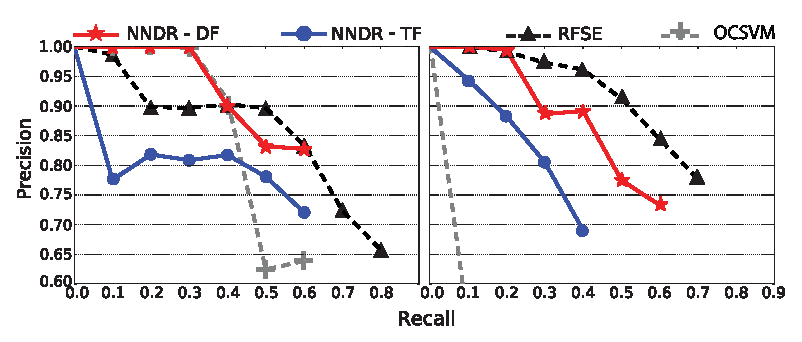
\includegraphics[scale=0.95]{Figures/NNDR_W3G-W1G_Best_RFSE-OCSVM-Baselines.eps}
	\caption{Precision curves in 11-standard recall levels of the examined open-set classifiers using either W3G features (left) or W1G features (right).}
	\label{chap:word_embeddings:fig:NNDR_W3G_Best_RFSE_Baseline}
	\end{center}
\end{figure}

%, i.e. the remaining part after the last mark of each curve it the percentage of the corpus tha has been classified as Unknown from the algorithms.

\section{Conclusions}\label{chap:word_embeddings:sec:conclusions}

In this chapter is presented an experimental study focused on WGI and the use of distributional features in combination with an open-set classifier that obtained promising results in other domains. Our experiments are based on a benchmark corpus already used in prior art and a strong baseline. Particularly it is evaluated the possible performance improvement of an open-set algorithm when distributional features are employed, using the SANTINIS corpus (i.e. a corpus with an unstructured noise).

It seems that distributional features provide a significant enhancement to the NNDR open-set method. The low-dimensionality of DF is crucial to boost the performance of NNDR. Yet, RFSE proves to be a hard-to-beat baseline at the expense of relying upon a much higher representation space (usually in the thousands of features). However, with respect to precision, the NNDR with PVBOW neural model input, is much more conservative and it prefers to leave web-pages unclassified rather than guessing an inaccurate genre label. Depending on the application of WGI, precision can be considered much more important than recall and this is where the proposed approach shines, i.e an open-set algorithm combined with \tetxit{neural language model}.

The open-set algorithm NNDR have been evaluated with distributional features which have been described in detail in chapter \ref{chap:openset}. A \textDistance Ration threshold is calculated while the training procedure for maximizing the \textit{Normalized Accuracy} of the known and the unknown classes.

The evaluation methodology previews shown to be proper for evaluation open-set scenarios. The natural focus in an open-set evaluation framework is the macro-precision, because always there is a part of the corpus will be classified as unknown. Either in the case of structured and unstructured or it is considered as outage while training.

Further research could focus on more appropriate distance measures within NNDR specially with recent data-driven features obtained with powerful NLP convolutional and recurrent deep networks. Moreover, alternative types of distributional features could be used (e.g., topic modeling). Finally, a combination of NNDR with RFSE models could be studied as they seem to exploit complementary views of the same problem.

